\documentclass[11pt,a4paper]{article}

\usepackage[a4paper,top=23mm,bottom=24mm,left=22mm,right=22mm,headheight=15pt]{geometry}
\usepackage[T1]{fontenc}
\usepackage[utf8]{inputenc}
\usepackage[provide=*,french]{babel}
\usepackage{newpxtext,newpxmath}
\usepackage[scaled=0.92]{sourcesanspro}
\usepackage[scaled=0.88]{inconsolata}

\usepackage[table]{xcolor}
\usepackage{microtype}
\usepackage{booktabs}
\usepackage{longtable}
\usepackage{tabularx}
\usepackage{array}
\usepackage{makecell}
\usepackage{enumitem}
\usepackage{titlesec}
\usepackage{fancyhdr}
\usepackage{graphicx}
\usepackage{float}
\usepackage{tikz}
\usetikzlibrary{arrows.meta,positioning,shapes.geometric,fit}
\usepackage[most]{tcolorbox}
\usepackage{caption}
\usepackage{hyperref}
\usepackage{bookmark}
\usepackage{csquotes}

\definecolor{Navy}{HTML}{17324D}
\definecolor{Teal}{HTML}{137C8B}
\definecolor{Gold}{HTML}{D89B2B}
\definecolor{Ice}{HTML}{EAF3F5}
\definecolor{Mist}{HTML}{F4F6F8}
\definecolor{Ink}{HTML}{27313A}
\definecolor{Muted}{HTML}{65727E}
\definecolor{Rule}{HTML}{CFD8DE}
\definecolor{SoftGold}{HTML}{FFF6DF}

\hypersetup{
  colorlinks=true,
  linkcolor=Navy,
  citecolor=Teal,
  urlcolor=Teal,
  pdftitle={Protocole ODD du modèle ABM de conformité organisationnelle},
  pdfsubject={Description structurée selon Overview, Design concepts and Details},
  pdfkeywords={ABM, ODD, conformité, influence sociale, sanctions, IEEE}
}

\pagestyle{fancy}
\fancyhf{}
\fancyhead[L]{\sffamily\small\color{Muted}Protocole ODD — modèle ABM}
\fancyhead[R]{\sffamily\small\color{Muted}Version 1.2}
\fancyfoot[L]{\sffamily\footnotesize\color{Muted}Modèle ABM de conformité organisationnelle}
\fancyfoot[R]{\sffamily\footnotesize\color{Muted}Page \thepage}
\renewcommand{\headrulewidth}{0.4pt}
\renewcommand{\footrulewidth}{0pt}

\titleformat{\section}
  {\sffamily\Large\bfseries\color{Navy}}
  {\thesection}{0.65em}{}
  [\vspace{0.25em}\color{Teal}\titlerule]
\titleformat{\subsection}
  {\sffamily\large\bfseries\color{Navy}}
  {\thesubsection}{0.55em}{}
\titleformat{\subsubsection}
  {\sffamily\normalsize\bfseries\color{Teal}}
  {\thesubsubsection}{0.5em}{}
\titlespacing*{\section}{0pt}{2.2ex plus 0.8ex}{1.2ex}
\titlespacing*{\subsection}{0pt}{1.8ex plus 0.5ex}{0.8ex}
\titlespacing*{\subsubsection}{0pt}{1.4ex plus 0.4ex}{0.5ex}

\setlist[itemize]{leftmargin=1.5em,itemsep=0.25em,topsep=0.35em}
\setlist[enumerate]{leftmargin=1.7em,itemsep=0.3em,topsep=0.4em}
\setlength{\parindent}{0pt}
\setlength{\parskip}{0.55em}
\setlength{\tabcolsep}{5pt}
\renewcommand{\arraystretch}{1.18}
\captionsetup{font=small,labelfont={bf,sf,color=Navy},textfont={color=Ink}}

\newcolumntype{Y}{>{\raggedright\arraybackslash}X}
\newcolumntype{C}[1]{>{\centering\arraybackslash}p{#1}}
\newcolumntype{L}[1]{>{\raggedright\arraybackslash}p{#1}}
\newcommand{\code}[1]{\texttt{\small #1}}
\newcommand{\R}{\mathbb{R}}
\newcommand{\Prob}{\mathbb{P}}
\newcommand{\ODD}{\textsc{odd}}

\newtcolorbox{keybox}[1][]{
  enhanced,
  breakable,
  colback=Ice,
  colframe=Teal,
  boxrule=0.7pt,
  arc=2mm,
  left=3mm,right=3mm,top=2mm,bottom=2mm,
  fonttitle=\sffamily\bfseries,
  coltitle=Navy,
  #1
}
\newtcolorbox{warningbox}[1][]{
  enhanced,
  breakable,
  colback=SoftGold,
  colframe=Gold,
  boxrule=0.7pt,
  arc=2mm,
  left=3mm,right=3mm,top=2mm,bottom=2mm,
  fonttitle=\sffamily\bfseries,
  coltitle=Navy,
  #1
}

\begin{document}

\hypersetup{pageanchor=false}
\begin{titlepage}
\thispagestyle{empty}
\begin{tikzpicture}[remember picture,overlay]
  \fill[Navy] (current page.north west) rectangle ([yshift=-104mm]current page.north east);
  \fill[Teal] ([yshift=-104mm]current page.north west) rectangle ([yshift=-108mm]current page.north east);
  \fill[Mist] ([yshift=-108mm]current page.north west) rectangle (current page.south east);
  \draw[Gold,line width=2.2pt]
    ([xshift=22mm,yshift=-26mm]current page.north west) --
    ([xshift=22mm,yshift=-53mm]current page.north west);
\end{tikzpicture}

\vspace*{17mm}
{\sffamily\small\bfseries\color{Gold}\MakeUppercase{Modélisation à base d’agents}\par}
\vspace{5mm}
{\sffamily\fontsize{28}{33}\selectfont\bfseries\color{white}
Protocole ODD du modèle ABM\\[1mm]
de conformité organisationnelle\par}
\vspace{7mm}
{\sffamily\large\color{white}
Personnalité, influence sociale, hiérarchie et environnement institutionnel\par}

\vspace{42mm}
\begin{tcolorbox}[
  width=\textwidth,
  colback=white,
  colframe=Rule,
  boxrule=0.8pt,
  arc=2mm,
  left=6mm,right=6mm,top=5mm,bottom=5mm]
{\sffamily\bfseries\color{Navy}But de l’étude}\par
\vspace{1mm}
Nous étudions l’évolution de la conformité dans une organisation en comparant
trois situations : sans règles, avec des règles sans sanctions, puis avec des
règles accompagnées de surveillance et de sanctions.
\end{tcolorbox}

\vfill
\begin{tabularx}{\textwidth}{@{}L{36mm}Y@{}}
\sffamily\bfseries\color{Navy}Version & 1.2\\
\sffamily\bfseries\color{Navy}Date & 27 juillet 2026\\
\sffamily\bfseries\color{Navy}Type de modèle & Modèle à base d’agents (ABM)\\
\sffamily\bfseries\color{Navy}Statut & Spécification prête pour l’implémentation du prototype\\
\end{tabularx}
\end{titlepage}

\hypersetup{pageanchor=true}
\pagenumbering{roman}

\section*{Résumé}
\addcontentsline{toc}{section}{Résumé}

Dans ce travail, nous construisons un modèle à base d’agents pour étudier la
conformité dans une organisation. Les agents représentent des employés et des
chefs. Ils possèdent des traits de personnalité continus, une adhésion
intrinsèque aux normes, une influençabilité, une sensibilité aux sanctions et
une mémoire. Leur décision dépend de ce qu’ils observent autour d’eux : le
comportement des collègues, celui du chef, la règle, leur expérience récente et
le risque de sanction qu’ils perçoivent.

Nous comparons trois phases : l’absence de règles, la présence de règles sans
sanctions, puis la présence de règles avec surveillance et sanctions graduées.
Nous ne fixons pas le résultat collectif à l’avance. Il apparaît à partir des
décisions individuelles et des interactions répétées. Pour l’expérience
principale, nous retenons 100 agents répartis dans dix services, 200 périodes et
au moins 30 réplications par phase. Les valeurs numériques utilisées dans la
simulation sont des paramètres expérimentaux. Elles ne sont pas présentées
comme des valeurs données par les auteurs cités.

\begin{keybox}[title=Question scientifique]
Que se passe-t-il réellement lorsque des individus différents, soumis à des
influences sociales et hiérarchiques, évoluent sous plusieurs régimes
institutionnels ? Nous cherchons à savoir \emph{si}, \emph{quand}, \emph{dans
quelles conditions} et \emph{pour quels agents} les règles, la surveillance et
les sanctions modifient la conformité collective.
\end{keybox}

\textbf{Mots-clés —} modèle à base d’agents, protocole ODD, conformité,
personnalité, influence sociale, hiérarchie, règles, surveillance, sanctions,
phénomènes émergents.

\newpage
\tableofcontents
\newpage
\listoftables
\addcontentsline{toc}{section}{Liste des tableaux}

\newpage
\pagenumbering{arabic}

\section{Organisation de la description du modèle}

Nous décrivons le modèle avec le protocole \ODD{}. Ce protocole organise la
présentation en trois parties : \emph{Overview}, \emph{Design concepts} et
\emph{Details} \cite{grimm2020}. Ces parties permettent de préciser les agents,
les mécanismes, l’ordre des opérations et les paramètres utilisés.

Notre simulation part des règles individuelles. Les résultats observés au
niveau de l’organisation viennent ensuite des interactions entre les agents
\cite{epstein1996}. Nous ne programmons donc pas directement un taux de
conformité final \cite{gilbert2005}.

\subsection{Trois niveaux de traçabilité}

Pour ne pas confondre la théorie et nos propres choix, nous séparons trois
catégories :

\begin{enumerate}
  \item \textbf{Fondement théorique} : la littérature justifie l’existence du
  mécanisme.
  \item \textbf{Choix de modélisation} : nous choisissons une manière de
  représenter ce mécanisme dans la simulation.
  \item \textbf{Paramètre expérimental} : nous choisissons une valeur de départ,
  puis nous la faisons varier.
\end{enumerate}

\begin{warningbox}[title=Règle d’interprétation]
Une référence peut justifier un mécanisme sans donner sa valeur numérique. Par
exemple, les travaux sur l’autorité justifient que le chef ait un poids
particulier. Ils ne disent pas qu’il influence toujours deux fois plus qu’un
collègue. Le rapport $w_h/w_c=2$ est donc notre valeur de départ et doit être
testé.
\end{warningbox}

\subsection{Choix retenus pour les points non précisés}

Pour pouvoir implémenter le modèle, nous retenons les choix suivants :

\begin{itemize}
  \item deux réseaux non orientés entre pairs : un réseau d’employés et un
  réseau de chefs, sans boucle ni arête multiple ;
  \item liens hiérarchiques séparés des liens entre pairs ;
  \item proportion attendue de liens internes au service fixée à
  $p_{\mathrm{intra}}=0{,}80$ pour les employés ;
  \item mise à jour synchrone des comportements afin d’éviter un avantage lié à
  l’ordre des agents ;
  \item initialisation neutre de la mémoire à $0{,}5$ et de la perception du
  risque à $0{,}5$ dans la phase sanctionnée ;
  \item centrage des prédicteurs continus par $c(x)=2x-1$ dans la fonction de
  décision.
\end{itemize}

Ces valeurs ne viennent pas directement de la littérature. Nous les gardons
comme choix de départ et nous testons leur effet dans l’analyse de sensibilité.

\begin{table}[H]
\centering
\caption{Décisions finales pour l’implémentation du prototype}
\label{tab:finalchoices}
\begin{tabularx}{\textwidth}{@{}L{36mm}L{49mm}Y@{}}
\toprule
\rowcolor{Navy}
\color{white}\textbf{Point à fixer} &
\color{white}\textbf{Choix retenu} &
\color{white}\textbf{Application}\\
\midrule
Mémoire &
Moyenne exponentielle, $\lambda=0{,}8$ &
Une seule variable $M_i(t)$ ; aucun historique complet n’est stocké.\\
Sanctions &
$(\ell_1,\ell_2,\ell_3)=(0{,}25;0{,}50;1{,}00)$ &
Avertissement, sanction modérée, puis sanction forte.\\
Réseau &
Employés reliés aux employés ; chefs reliés aux chefs &
Le lien chef--employé reste un lien hiérarchique distinct.\\
Observations &
Agent lui-même, voisins directs et chef pour les employés &
Les comportements et les sanctions visibles viennent de la période précédente.\\
Sanction attendue &
Niveau de la prochaine violation détectée &
$\widehat L_i(t)$ dépend de $V_i(t-1)$.\\
Implémentation &
Python 3.12.3, bibliothèque standard &
Une graine et un fichier de configuration sont enregistrés par exécution.\\
\bottomrule
\end{tabularx}
\end{table}

\section{Overview — Vue d’ensemble}

\subsection{Objectif et motifs à reproduire}

\subsubsection{Objectif}

Nous cherchons à observer comment la conformité évolue sous l’effet combiné :

\begin{itemize}
  \item des différences individuelles ;
  \item de l’observation des collègues et des chefs ;
  \item des interactions répétées et de la mémoire ;
  \item de la présence d’une règle ;
  \item de la surveillance, de la détection et de sanctions graduées.
\end{itemize}

Nous partons des décisions individuelles, puis nous observons la dynamique
collective. Nous ne supposons donc pas au départ que
$TC_{\mathrm{phase\,3}}>TC_{\mathrm{phase\,2}}>TC_{\mathrm{phase\,1}}$.

\subsubsection{Résultats que nous voulons observer}

Nous ne disposons pas encore de données empiriques pour fixer des valeurs
cibles. Nous regarderons surtout si les phénomènes suivants apparaissent :

\begin{itemize}
  \item apparition possible d’une norme locale dominante sans règle formelle ;
  \item hétérogénéité persistante entre services ;
  \item accélération ou freinage de la diffusion par le comportement du chef ;
  \item hausse de la conformité lorsque le risque perçu de sanction augmente,
  sans réponse déterministe ;
  \item inertie, résistance locale, convergence ou polarisation selon la
  structure du réseau et les profils d’agents ;
  \item persistance possible d’une norme informelle malgré l’introduction d’une
  règle officielle.
\end{itemize}

\subsection{Entités, variables d’état et échelles}

\subsubsection{Entités}

Nous utilisons trois niveaux :

\begin{enumerate}
  \item \textbf{Agents} : employés et chefs, qui peuvent adopter un
  comportement conforme ou non conforme.
  \item \textbf{Services} : chaque service regroupe un chef et des employés.
  \item \textbf{Organisation} : elle regroupe toute la population,
  l’environnement institutionnel et les indicateurs globaux.
\end{enumerate}

Dans la configuration de référence :
\[
N=100,\qquad N_E=90,\qquad N_H=10,\qquad G=10,
\]
soit un chef et neuf employés par service.

\subsubsection{Variables individuelles}

\begin{longtable}{L{31mm}L{34mm}L{72mm}}
\caption{Variables d’état d’un agent}\label{tab:state}\\
\toprule
\rowcolor{Navy}
\color{white}\textbf{Variable} &
\color{white}\textbf{Domaine} &
\color{white}\textbf{Interprétation}\\
\midrule
\endfirsthead
\toprule
\rowcolor{Navy}
\color{white}\textbf{Variable} &
\color{white}\textbf{Domaine} &
\color{white}\textbf{Interprétation}\\
\midrule
\endhead
$O_i,C_i,E_i,A_i,N_i$ & $[0,1]^5$ &
Ouverture, conscienciosité, extraversion, agréabilité et neuroticisme.\\
$I_i$ & $[0,1]$ & Influençabilité ou sensibilité aux signaux sociaux.\\
$K_i$ & $[0,1]$ & Adhésion intrinsèque à la norme.\\
$S_i$ & $[0,1]$ & Sensibilité individuelle aux sanctions.\\
$H_i$ & $\{w_c,w_h\}$ & Poids d’autorité associé au rôle de l’agent.\\
$M_i(t)$ & $[0,1]$ & Mémoire comportementale décroissante.\\
$\widehat p_i(t)$ & $[0,1]$ & Probabilité de détection perçue.\\
$V_i(t)$ & $\mathbb{N}$ & Nombre cumulé de violations détectées.\\
$B_i(t)$ & $\{0,1\}$ & Comportement : 1 conforme, 0 non conforme.\\
$P_i^{(c)}(t)$ & $[0,1]$ & Probabilité instantanée d’adopter le comportement conforme.\\
$g_i$ & $\{1,\ldots,G\}$ & Service d’appartenance.\\
$r_i$ & \{employé, chef\} & Rôle organisationnel.\\
$\mathcal{N}_i$ & ensemble & Voisins sociaux observables par l’agent.\\
\bottomrule
\end{longtable}

L’état compact d’un agent s’écrit :
\[
\mathcal{A}_i(t)=
\bigl(O_i,C_i,E_i,A_i,N_i,I_i,K_i,S_i,H_i,M_i(t),
\widehat p_i(t),V_i(t),B_i(t),g_i,r_i,\mathcal{N}_i\bigr).
\]

\subsubsection{Échelles temporelle et structurelle}

Une période représente un cycle abstrait d’observation, de décision et de
réaction institutionnelle. Aucune correspondance calendaire n’est imposée tant
qu’elle n’a pas été reliée à des données empiriques. La simulation de référence
dure $T=200$ périodes ; la sensibilité est examinée de 100 à 1\,000 périodes.

Le modèle ne comporte pas d’espace géographique. L’espace pertinent est un
réseau multiplexe :

\begin{itemize}
  \item liens sociaux entre pairs ;
  \item lien hiérarchique dirigé du chef vers les employés de son service ;
  \item appartenance commune à un service.
\end{itemize}

\subsection{Vue générale des processus et ordonnancement}

La mise à jour est synchrone : toutes les décisions à la période $t$ utilisent
les comportements de $t-1$. Les nouveaux comportements sont appliqués
simultanément.

\begin{figure}[htbp]
\centering
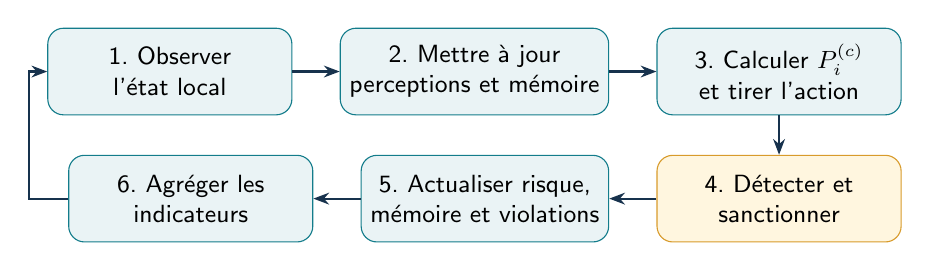
\begin{tikzpicture}[
  node distance=5mm and 6mm,
  every node/.style={font=\sffamily\small},
  process/.style={rectangle,rounded corners=2mm,draw=Teal,fill=Ice,
    minimum width=31mm,minimum height=11mm,align=center},
  inst/.style={rectangle,rounded corners=2mm,draw=Gold,fill=SoftGold,
    minimum width=31mm,minimum height=11mm,align=center},
  arrow/.style={-{Stealth[length=2mm]},thick,color=Navy}
]
\node[process] (obs) {1. Observer\\l’état local};
\node[process,right=of obs] (per) {2. Mettre à jour\\perceptions et mémoire};
\node[process,right=of per] (dec) {3. Calculer $P_i^{(c)}$\\et tirer l’action};
\node[inst,below=of dec] (mon) {4. Détecter et\\sanctionner};
\node[process,left=of mon] (mem) {5. Actualiser risque,\\mémoire et violations};
\node[process,left=of mem] (agg) {6. Agréger les\\indicateurs};
\draw[arrow] (obs)--(per);
\draw[arrow] (per)--(dec);
\draw[arrow] (dec)--(mon);
\draw[arrow] (mon)--(mem);
\draw[arrow] (mem)--(agg);
\draw[arrow] (agg.west) -- ++(-5mm,0) |- (obs.west);
\end{tikzpicture}
\caption{Cycle d’une période de simulation}
\label{fig:schedule}
\end{figure}

À $t=0$, la population, le réseau, les caractéristiques et les comportements
initiaux sont générés. Pour chaque $t=1,\ldots,T$ :

\begin{enumerate}
  \item les agents observent les comportements précédents de leurs voisins et,
  pour les employés, de leur chef, ainsi que les sanctions visibles ;
  \item l’influence sociale, la mémoire et le risque de détection perçu sont
  mis à jour ;
  \item chaque agent calcule une probabilité de conformité et effectue un tirage
  de Bernoulli ;
  \item si la surveillance est active, les violations sont détectées avec la
  probabilité réelle $p_d$ et reçoivent une sanction graduée ;
  \item les compteurs et perceptions sont actualisés ;
  \item les sorties individuelles, par service et globales sont enregistrées.
\end{enumerate}

\section{Design concepts — Concepts de conception}

\subsection{Principes de base}

\subsubsection{Personnalité}

Nous représentons la personnalité avec les cinq dimensions OCEAN
\cite{costa1992}. Nous les gardons continues et nous ne les utilisons jamais
pour décider directement qu’un agent sera conforme ou non conforme. Les valeurs
dans $[0,1]$ servent seulement à faciliter les calculs.

\subsubsection{Apprentissage social et influence}

Un agent peut changer sa décision après avoir observé le comportement des autres
et ses conséquences \cite{bandura1977}. Nous utilisons la preuve sociale pour
représenter l’effet de la majorité locale et l’autorité pour donner un poids
particulier au chef \cite{cialdini2009}. Les poids numériques restent nos
paramètres de simulation.

\subsubsection{Rationalité limitée}

Les agents ne connaissent pas l’état complet de l’organisation. Ils décident
avec les informations locales qu’ils perçoivent. Ce choix reprend le principe
de rationalité limitée dans les organisations \cite{simon1997}.

\subsubsection{Institutions, interactions répétées et émergence}

Nous séparons la règle, la surveillance et la sanction. Les sanctions deviennent
plus fortes lorsque les violations détectées se répètent
\cite{ostrom1990}. Nous ajoutons aussi une mémoire parce que les agents se
rencontrent plusieurs fois \cite{axelrod2006}. Les comportements collectifs
sont ensuite calculés à partir des décisions locales, selon la logique
micro--macro de Schelling \cite{schelling2006}.

\subsection{Émergence}

Le modèle doit faire apparaître, sans les fixer à l’avance :

\begin{itemize}
  \item le taux de conformité global et par service ;
  \item les normes locales ;
  \item la convergence, l’instabilité ou la polarisation ;
  \item les groupes comportementaux ;
  \item la résistance à une majorité locale ;
  \item les profils a posteriori : conformiste social, conformiste
  institutionnel, résistant intrinsèque ou non-conformiste persistant.
\end{itemize}

Nous n’attribuons pas ces profils au début de la simulation. Nous les
identifions après avoir observé les trajectoires des agents.

\subsection{Adaptation}

Un agent peut s’adapter de trois manières :

\begin{enumerate}
  \item ajustement probabiliste au comportement local ;
  \item évolution de la mémoire par pondération décroissante du passé ;
  \item révision du risque perçu après sanctions personnelles ou observées.
\end{enumerate}

Dans la version de référence, les traits OCEAN, l’adhésion intrinsèque et
l’influençabilité restent fixes pendant une exécution.

\subsection{Objectifs individuels}

Nous ne donnons pas aux agents une fonction d’utilité globale à maximiser. La
valeur $Z_i(t)$ combine leurs dispositions personnelles, les signaux sociaux et
les signaux institutionnels. La décision dépend donc des informations
disponibles et non d’une connaissance parfaite du système.

\subsection{Apprentissage}

Nous représentons l’apprentissage par le risque perçu $\widehat p_i(t)$ et par
la mémoire $M_i(t)$. La personnalité ne change pas pendant la simulation. Dans
une autre version du modèle, nous pourrons aussi faire évoluer $K_i$ ou $I_i$,
mais ce mécanisme n’est pas retenu ici.

\subsection{Prédiction}

Pour décider, les agents utilisent le comportement récent et le risque qu’ils
perçoivent. Ils ne connaissent pas directement $p_d$ et ne calculent pas les
intentions des autres agents. Ainsi :
\[
p_d \neq \widehat p_i(t)
\]
en général.

\subsection{Perception}

À la période $t$, un agent utilise les observations faites à la période
$t-1$. Il perçoit :

\begin{itemize}
  \item le comportement de tous ses voisins directs ;
  \item le comportement de son chef s’il est employé ;
  \item la règle communiquée ;
  \item ses propres sanctions ;
  \item la présence ou l’absence de sanction après une violation commise par un
  voisin direct ;
  \item la sanction éventuelle de son chef s’il est employé.
\end{itemize}

Toutes les observations du voisinage direct sont donc visibles. L’agent ne voit
pas les comportements ni les sanctions situés en dehors de ce voisinage. Il ne
connaît pas non plus les intentions des autres agents ni le paramètre réel de
détection.

\subsection{Interaction}

Un voisin influence un agent par son comportement observé. Le chef possède un
poids plus élevé dans cette influence. Dans cette version du modèle, les agents
ne négocient pas, n’échangent pas de ressources et ne s’envoient pas de messages
argumentés.

\subsection{Stochasticité}

La stochasticité intervient dans :

\begin{itemize}
  \item la génération des traits et dispositions ;
  \item la construction du réseau ;
  \item le comportement initial ;
  \item le tirage de chaque comportement ;
  \item la détection d’une violation ;
  \item le bruit comportemental $\varepsilon_i(t)$.
\end{itemize}

Les graines pseudo-aléatoires sont enregistrées et appariées entre scénarios.

\subsection{Collectifs}

Les services sont fixés à l’initialisation. Les groupes comportementaux sont
détectés après simulation à partir de la similarité des trajectoires et/ou de la
structure du réseau. Aucun collectif comportemental n’est imposé.

\subsection{Observation}

Les variables sont enregistrées à chaque période au niveau individuel, au
niveau du service et au niveau de l’organisation. Les sorties primaires sont
détaillées au tableau~\ref{tab:outputs}.

\begin{longtable}{L{37mm}L{44mm}L{61mm}}
\caption{Indicateurs de sortie}\label{tab:outputs}\\
\toprule
\rowcolor{Navy}
\color{white}\textbf{Indicateur} &
\color{white}\textbf{Définition opérationnelle} &
\color{white}\textbf{Usage}\\
\midrule
\endfirsthead
\toprule
\rowcolor{Navy}
\color{white}\textbf{Indicateur} &
\color{white}\textbf{Définition opérationnelle} &
\color{white}\textbf{Usage}\\
\midrule
\endhead
Conformité globale &
$TC(t)=N^{-1}\sum_i B_i(t)$ &
Dynamique macroscopique centrale.\\
Conformité moyenne &
$\overline{TC}=T^{-1}\sum_t TC(t)$ &
Comparaison synthétique des scénarios.\\
Conformité par service &
$TC_g(t)=N_g^{-1}\sum_{i:g_i=g}B_i(t)$ &
Hétérogénéité organisationnelle.\\
Variabilité interservices &
$\operatorname{Var}_g[TC_g(t)]$ &
Dispersion et polarisation locale.\\
Transitions &
$\sum_{i,t}\mathbf{1}[B_i(t)\neq B_i(t-1)]$ &
Instabilité comportementale.\\
Résistance sociale &
Part des agents conservant leur état malgré une majorité locale opposée &
Persistance individuelle.\\
Effet du chef &
Différence de conformité des employés selon $B_{\mathrm{chef}}(t-1)$ &
Influence hiérarchique conditionnelle.\\
Convergence &
Premier $t_0$ tel que $|TC(t)-TC(t-1)|<0{,}01$ durant dix périodes &
Vitesse de stabilisation ; seuil à tester.\\
Polarisation &
Coexistence de services à $TC_g\leq0{,}20$ et $TC_g\geq0{,}80$ &
Extrêmes simultanés ; seuils à tester.\\
Violations détectées &
$\sum_{i,t}\mathbf{1}[B_i(t)=0\land D_i(t)=1]$ &
Intensité d’application institutionnelle.\\
\bottomrule
\end{longtable}

\section{Details — Détails d’implémentation}

\subsection{Initialisation}

\subsubsection{Population et services}

Pour l’expérience principale, nous retenons dix services. Chaque service
contient un chef et neuf employés. Les chefs prennent leurs décisions avec les
mêmes mécanismes que les employés. Leur rôle change surtout leur position dans
le réseau et leur poids d’autorité.

\subsubsection{Réseau social}

Nous construisons séparément le réseau des employés et celui des chefs. Il
n’existe pas de lien de pair entre un employé et un chef. Cette relation est
représentée uniquement par le lien hiérarchique.

Pour chaque employé, nous tirons un degré cible :
\[
k_i^{E}\sim\mathcal{U}\{4,5,6,7,8\}.
\]
Lors de la création d’un lien, nous cherchons un autre employé du même service
avec une probabilité $p_{\mathrm{intra}}=0{,}80$. Avec une probabilité de
$0{,}20$, nous cherchons un employé d’un autre service. Si aucun candidat n’est
disponible dans le groupe choisi, nous utilisons l’autre groupe.

Les chefs possèdent aussi un réseau entre pairs. Comme il n’y a qu’un chef par
service, leurs relations sont nécessairement interservices :
\[
k_i^{H}\sim\mathcal{U}\{4,\ldots,\min(8,N_H-1)\}.
\]
Cette formule s’applique lorsque $N_H\geq5$. Si $2\leq N_H<5$, chaque chef est
relié aux $N_H-1$ autres chefs. Si $N_H=1$, son voisinage de pairs est vide.

Pour les deux réseaux, nous appliquons le même algorithme :

\begin{enumerate}
  \item nous créons pour chaque agent un nombre de places libres égal à son
  degré cible ;
  \item nous choisissons l’agent qui possède le plus de places libres ; les
  égalités sont départagées aléatoirement ;
  \item nous choisissons un candidat ayant encore une place libre, sans boucle
  et sans lien déjà existant ;
  \item nous ajoutons le lien et nous diminuons les deux compteurs ;
  \item si l’algorithme se bloque avant d’atteindre tous les degrés, nous
  recommençons la construction ; après 100 échecs, nous retirons une nouvelle
  séquence de degrés.
\end{enumerate}

Les liens entre pairs sont non orientés. Le réseau final et la séquence de
degrés sont enregistrés avec les résultats. En plus du réseau des employés,
chaque employé observe le chef de son service par un lien hiérarchique dirigé.

Les poids de référence sont :
\[
w_c=1 \quad\text{pour un pair},\qquad
w_h=2 \quad\text{pour le chef}.
\]

\subsubsection{Caractéristiques}

Tant que nous ne disposons pas de données empiriques, nous générons séparément
les traits OCEAN, l’influençabilité, l’adhésion intrinsèque et la sensibilité aux
sanctions :
\[
O_i,C_i,E_i,A_i,N_i,I_i,K_i,S_i\sim\operatorname{Beta}(2,2).
\]
La loi $\operatorname{Beta}(2,2)$ produit davantage de valeurs intermédiaires
mais permet aussi d’obtenir des valeurs faibles et élevées. Ce choix reste une
hypothèse de simulation. Nous le remplacerons par les distributions observées
si nous obtenons des données.

\subsubsection{État dynamique initial}

On pose :
\[
M_i(0)=0{,}5,\qquad V_i(0)=0.
\]
Dans les phases 1 et 2, nous posons $\widehat p_i(0)=0$. Dans la phase 3, nous
commençons avec $\widehat p_i(0)=0{,}5$. Nous réutilisons les mêmes agents, les
mêmes traits, le même réseau et les mêmes graines dans les trois phases.

Le comportement initial est tiré avec les seuls déterminants individuels :
\[
B_i(0)\sim\operatorname{Bernoulli}\!\left(
\sigma\left[\beta_0+\beta_P P_i+\beta_Kc(K_i)+\varepsilon_i(0)\right]
\right),
\]
où $\sigma(z)=(1+e^{-z})^{-1}$ et $c(x)=2x-1$.

\subsection{Données d’entrée}

Dans la première version, nous n’utilisons pas de série temporelle externe. Les
entrées sont :

\begin{itemize}
  \item un fichier de configuration des paramètres ;
  \item une liste de graines pseudo-aléatoires ;
  \item les indicateurs de scénario
  \code{rules\_enabled}, \code{monitoring\_enabled} et
  \code{sanctions\_enabled}.
\end{itemize}

Si nous obtenons des données organisationnelles, nous pourrons remplacer la
population synthétique, les distributions des traits, le réseau, le taux
initial de conformité et les paramètres de détection. Nous préciserons alors
l’unité de chaque donnée, sa période, le traitement des valeurs manquantes et
son lien avec les agents.

\subsubsection{Environnement d’implémentation}

Nous retenons Python 3.12.3 et la bibliothèque standard. Cette solution suffit
pour la population et la durée prévues et évite de rendre le prototype dépendant
d’un cadre ABM particulier. Les principaux modules utilisés seront
\code{random}, \code{math}, \code{json}, \code{csv}, \code{statistics},
\code{dataclasses} et \code{pathlib}.

Chaque exécution utilise sa propre instance \code{random.Random(seed)}. Nous
n’utilisons pas le générateur aléatoire global. Le dossier d’une exécution
contient au minimum :

\begin{itemize}
  \item \code{configuration.json} : paramètres et graine ;
  \item \code{agents.csv} : caractéristiques initiales des agents ;
  \item \code{network.csv} : liens entre pairs et liens hiérarchiques ;
  \item \code{timeseries.csv} : indicateurs par période et par service ;
  \item \code{events.csv} : violations, détections et sanctions.
\end{itemize}

\subsection{Sous-modèles}

\subsubsection{Contribution de la personnalité}

Nous centrons et nous bornons la contribution de la personnalité :
\[
P_i=
\frac{\alpha_Oc(O_i)+\alpha_Cc(C_i)+\alpha_Ec(E_i)
+\alpha_Ac(A_i)+\alpha_Nc(N_i)}
{\sum_{q\in\{O,C,E,A,N\}}|\alpha_q|}.
\]
Si tous les $\alpha_q$ sont nuls, $P_i=0$. Pour la configuration de départ, nous
utilisons
\[
(\alpha_O,\alpha_C,\alpha_E,\alpha_A,\alpha_N)=(0,1,0,1,-1).
\]
Nous enregistrons toujours l’ouverture et l’extraversion, mais elles n’agissent
pas dans la configuration de départ. Leur effet devra d’abord être mieux
justifié. Tous les $\alpha_q$ restent à calibrer.

\subsubsection{Influence sociale et autorité}

L’influence observée est la moyenne pondérée des comportements antérieurs :
\[
SI_i(t)=
\frac{\displaystyle\sum_{j\in\mathcal{N}_i}w_{ij}B_j(t-1)
+\mathbf{1}_{\{r_i=\text{employé}\}}w_hB_{h(i)}(t-1)}
{\displaystyle\sum_{j\in\mathcal{N}_i}w_{ij}
+\mathbf{1}_{\{r_i=\text{employé}\}}w_h},
\]
où $h(i)$ est le chef de l’employé $i$ et $w_{ij}=w_c$ dans le scénario de
référence. Le terme social dans la décision est $I_i\,c(SI_i(t))$.

\begin{warningbox}[title=Absence de double comptage de l’autorité]
L’autorité est intégrée dans $SI_i(t)$ par le poids $w_h$. Aucun second terme
d’autorité n’est ajouté dans la fonction centrale. Une extension qui introduit
un coefficient $\beta_A$ séparé doit retirer le chef de la moyenne sociale ou
fixer l’un des deux effets à zéro.
\end{warningbox}

\subsubsection{Mémoire}

La mémoire résume la persistance du comportement récent :
\[
M_i(t)=\lambda M_i(t-1)+(1-\lambda)B_i(t-1),
\qquad 0\leq\lambda\leq1.
\]
Nous retenons uniquement cette mémoire exponentielle avec $\lambda=0{,}8$. Les
dix dernières périodes représentent alors environ
$1-0{,}8^{10}=89{,}3\,\%$ du poids des observations. Nous ne stockons pas de
fenêtre glissante séparée.

\subsubsection{Règle, surveillance et sanctions}

Les trois environnements sont définis au tableau~\ref{tab:phases}.

\begin{table}[htbp]
\centering
\caption{Configuration des phases expérimentales}
\label{tab:phases}
\begin{tabularx}{\textwidth}{@{}L{38mm}C{16mm}C{25mm}C{18mm}Y@{}}
\toprule
\rowcolor{Navy}
\color{white}\textbf{Phase} &
\color{white}\textbf{Règle} &
\color{white}\textbf{Surveillance} &
\color{white}\textbf{Sanction} &
\color{white}\textbf{Effets actifs}\\
\midrule
1 — Absence de règles & Non & Non & Non &
Personnalité, adhésion, influence et mémoire.\\
2 — Règles seules & Oui & Non & Non &
Effets précédents + règle perçue.\\
3 — Régime complet & Oui & Oui & Oui &
Effets précédents + risque et sanctions graduées.\\
\bottomrule
\end{tabularx}
\end{table}

La règle perçue vaut $R_i(t)=0$ en phase 1 et $R_i(t)=1$ dans les phases 2 et
3, car la règle est communiquée à tous les agents. Lorsqu’une violation a lieu
en phase 3 :
\[
D_i(t)\sim\operatorname{Bernoulli}(p_d).
\]
Si l’agent est conforme, nous posons $D_i(t)=0$. Si une violation est détectée,
le compteur devient $V_i(t)=V_i(t-1)+1$ et la sanction appliquée est :
\[
L_i(t)=
\begin{cases}
0{,}25,&V_i(t)=1 \quad\text{(avertissement)},\\
0{,}50,&V_i(t)=2 \quad\text{(sanction modérée)},\\
1{,}00,&V_i(t)\geq3 \quad\text{(sanction forte)}.
\end{cases}
\]
Ainsi,
\[
(\ell_1,\ell_2,\ell_3)=(0{,}25;0{,}50;1{,}00).
\]
Si la violation n’est pas détectée, le compteur ne change pas et $L_i(t)=0$.
Aucune sanction n’est déclenchée en phase 1 ou 2.

\subsubsection{Risque perçu}

Soit $X_i^{\mathrm{pers}}(t-1)$ le résultat informatif d’une violation
personnelle : 1 si détectée, 0 si non détectée, et $\widehat p_i(t-1)$ si
l’agent n’a pas violé. Soit $X_i^{\mathrm{obs}}(t-1)$ le ratio de violations
détectées parmi les violations observées chez ses voisins directs et, pour un
employé, chez son chef. En l’absence d’observation pertinente, il est remplacé
par $\widehat p_i(t-1)$. Alors :
\[
\widehat p_i(t)=
\alpha X_i^{\mathrm{pers}}(t-1)
+\gamma X_i^{\mathrm{obs}}(t-1)
+(1-\alpha-\gamma)\widehat p_i(t-1),
\]
avec $\alpha,\gamma\geq0$ et $\alpha+\gamma\leq1$. Nous retenons
$\alpha=\gamma=0{,}4$. Le signal anticipé de sanction est :
\[
SR_i(t)=S_i\,\widehat p_i(t)\,\widehat L_i(t),
\]
où le niveau attendu est celui de la prochaine violation détectée :
\[
\widehat L_i(t)=
\begin{cases}
0{,}25,&V_i(t-1)=0,\\
0{,}50,&V_i(t-1)=1,\\
1{,}00,&V_i(t-1)\geq2.
\end{cases}
\]
L’agent connaît son nombre de violations déjà détectées, mais il utilise
$\widehat p_i(t)$ et non le risque réel $p_d$.

\subsubsection{Décision comportementale}

À chaque période, la valeur latente est :
\[
\begin{aligned}
Z_i(t)=\;&\beta_0+\beta_PP_i+\beta_Kc(K_i)
+\beta_I I_i\,c(SI_i(t))\\
&+\beta_RR_i(t)+\beta_SSR_i(t)
+\beta_Mc(M_i(t))+\varepsilon_i(t).
\end{aligned}
\]
Elle devient une probabilité :
\[
P_i^{(c)}(t)=\sigma[Z_i(t)]
=\frac{1}{1+\exp[-Z_i(t)]}.
\]
Enfin :
\[
u_i(t)\sim\mathcal{U}(0,1),\qquad
B_i(t)=
\begin{cases}
1,&u_i(t)<P_i^{(c)}(t),\\
0,&\text{sinon}.
\end{cases}
\]
Le comportement reste ainsi probabiliste : une règle ou une sanction augmente
éventuellement la probabilité de conformité sans la garantir.

\subsubsection{Coefficients de référence}

\begin{table}[htbp]
\centering
\caption{Coefficients de la fonction de décision}
\label{tab:coeff}
\begin{tabularx}{\textwidth}{@{}L{37mm}C{27mm}Y@{}}
\toprule
\rowcolor{Navy}
\color{white}\textbf{Terme} &
\color{white}\textbf{Référence} &
\color{white}\textbf{Statut}\\
\midrule
Intercept $\beta_0$ & 0,0 & Retenu pour un point de départ neutre.\\
Personnalité $\beta_P$ & 0,5 & Paramètre expérimental.\\
Adhésion intrinsèque $\beta_K$ & 1,0 & Paramètre expérimental.\\
Influence sociale $\beta_I$ & 1,0 & Paramètre expérimental.\\
Règle $\beta_R$ & 0,7 & Paramètre expérimental.\\
Risque de sanction $\beta_S$ & 1,0 & Paramètre expérimental.\\
Mémoire $\beta_M$ & 0,6 & Paramètre expérimental.\\
Bruit $\varepsilon_i(t)$ & $\operatorname{Unif}(-0{,}2;0{,}2)$ &
Variation individuelle non expliquée.\\
\bottomrule
\end{tabularx}
\end{table}

\section{Plan expérimental et analyse}

\subsection{Expérience principale}

Entre les trois phases, nous gardons les mêmes agents, les mêmes traits, le même
réseau, les mêmes chefs et les mêmes graines. Seul l’environnement
institutionnel change. Nous calculons :
\[
\Delta_R=\overline{TC}_{2}-\overline{TC}_{1},
\qquad
\Delta_{MS}=\overline{TC}_{3}-\overline{TC}_{2}.
\]
$\Delta_R$ mesure la différence produite par l’introduction de la règle dans la
simulation. $\Delta_{MS}$ mesure la différence supplémentaire produite par la
surveillance et les sanctions. Ces résultats concernent d’abord le modèle. Ils
ne suffisent pas, à eux seuls, pour conclure à un effet causal dans une
organisation réelle.

\subsection{Réplications et graines}

Nous exécutons chaque configuration avec au moins 30 graines. Pour une
réplication donnée, nous utilisons la même graine dans les trois phases. Cette
technique de nombres aléatoires communs améliore la comparaison des scénarios
\cite{schruben2011}. Pour la réplication $r$ :
\[
\mathrm{seed}_{1,r}=\mathrm{seed}_{2,r}=\mathrm{seed}_{3,r}.
\]
Pour la configuration de référence, nous retenons les 30 graines entières
\[
\mathcal{S}=\{42,43,\ldots,71\}.
\]

Pour chaque indicateur, nous calculons la moyenne, l’écart-type, l’intervalle de
confiance et les différences appariées. Nous gardons aussi les trajectoires
temporelles au lieu de regarder uniquement la dernière période.

\subsection{Analyse de sensibilité}

\begin{longtable}{L{43mm}C{24mm}C{24mm}C{24mm}}
\caption{Paramètres expérimentaux de référence et plages de sensibilité}
\label{tab:params}\\
\toprule
\rowcolor{Navy}
\color{white}\textbf{Paramètre} &
\color{white}\textbf{Bas} &
\color{white}\textbf{Référence} &
\color{white}\textbf{Haut}\\
\midrule
\endfirsthead
\toprule
\rowcolor{Navy}
\color{white}\textbf{Paramètre} &
\color{white}\textbf{Bas} &
\color{white}\textbf{Référence} &
\color{white}\textbf{Haut}\\
\midrule
\endhead
Population $N$ & 50 & 100 & 500\\
Part des chefs & 5\,\% & 10\,\% & 20\,\%\\
Relations des employés $k^E$ & 2 & 4--8 & 12\\
Relations des chefs $k^H$ & 2 & 4--8 & 8\\
Liens internes des employés $p_{\mathrm{intra}}$ & 0,60 & 0,80 & 1,00\\
Poids collègue $w_c$ & 0,5 & 1,0 & 1,5\\
Poids chef $w_h$ & 1,0 & 2,0 & 3,0\\
Durée $T$ & 100 & 200 & 1\,000\\
Persistance $\lambda$ & 0,2 & 0,8 & 0,95\\
Poids personnalité $\beta_P$ & 0,2 & 0,5 & 1,0\\
Poids adhésion $\beta_K$ & 0,5 & 1,0 & 1,5\\
Poids influence $\beta_I$ & 0,5 & 1,0 & 2,0\\
Poids règle $\beta_R$ & 0,2 & 0,7 & 1,5\\
Poids sanction $\beta_S$ & 0,5 & 1,0 & 2,0\\
Poids mémoire $\beta_M$ & 0,2 & 0,6 & 1,5\\
Détection $p_d$ & 0,1 & 0,5 & 0,9\\
Première sanction $\ell_1$ & 0,10 & 0,25 & 0,40\\
Deuxième sanction $\ell_2$ & 0,30 & 0,50 & 0,70\\
Sanction forte $\ell_3$ & 0,60 & 1,00 & 1,00\\
\bottomrule
\end{longtable}

Nous commençons par faire varier un paramètre à la fois pour comprendre son
effet. Ensuite, nous faisons varier ensemble les paramètres les plus importants,
car l’autorité, l’influençabilité, la détection et la mémoire peuvent interagir.

\subsection{Comparaisons hiérarchiques}

Quatre contextes locaux sont suivis :
\[
\begin{array}{ll}
\text{chef conforme + groupe conforme},&
\text{chef conforme + groupe non conforme},\\
\text{chef non conforme + groupe conforme},&
\text{chef non conforme + groupe non conforme}.
\end{array}
\]
Ils permettent d’évaluer si l’autorité accélère une tendance déjà dominante ou
renverse une norme locale.

\section{Traçabilité, vérification et limites}

\subsection{Matrice de traçabilité scientifique}

\begin{longtable}{L{30mm}L{42mm}L{45mm}L{29mm}}
\caption{Traçabilité des principaux mécanismes}\label{tab:trace}\\
\toprule
\rowcolor{Navy}
\color{white}\textbf{Élément} &
\color{white}\textbf{Fondement} &
\color{white}\textbf{Traduction ABM} &
\color{white}\textbf{Valeurs}\\
\midrule
\endfirsthead
\toprule
\rowcolor{Navy}
\color{white}\textbf{Élément} &
\color{white}\textbf{Fondement} &
\color{white}\textbf{Traduction ABM} &
\color{white}\textbf{Valeurs}\\
\midrule
\endhead
Personnalité &
Big Five \cite{costa1992} &
Cinq traits continus ; effet indirect &
À calibrer\\
Observation sociale &
Bandura \cite{bandura1977} &
Comportements et conséquences observés &
Structure théorique\\
Preuve sociale &
Cialdini \cite{cialdini2009} &
Moyenne locale pondérée &
Poids à tester\\
Autorité &
Cialdini \cite{cialdini2009} &
Poids supérieur du chef &
$w_h/w_c$ expérimental\\
Information limitée &
Simon \cite{simon1997} &
Voisinage local et perceptions &
Choix structurel\\
Règle &
Ostrom \cite{ostrom1990} &
Variable séparée de la surveillance &
Manipulation\\
Détection &
Ostrom \cite{ostrom1990} &
Bernoulli de paramètre $p_d$ &
Expérimental\\
Sanctions graduées &
Ostrom \cite{ostrom1990} &
Niveaux $0{,}25$, $0{,}50$ et $1{,}00$ selon les violations détectées &
Référence à tester\\
Mémoire &
Axelrod \cite{axelrod2006} &
Moyenne exponentielle, $\lambda=0{,}8$ &
$\lambda$ à tester\\
Micro--macro &
Schelling \cite{schelling2006} &
Agrégation après décisions locales &
Émergent\\
Démarche générative &
Epstein et Axtell \cite{epstein1996} &
Règles locales vers motifs globaux &
Principe méthodologique\\
Documentation &
Grimm et al. \cite{grimm2020} &
Structure ODD en sept rubriques &
Standard descriptif\\
\bottomrule
\end{longtable}

\subsection{Vérification}

Avant d’interpréter les résultats, nous vérifions les cas suivants :

\begin{itemize}
  \item $p_d=0$ ne produit aucune sanction ;
  \item \code{rules\_enabled=false} impose $R_i(t)=0$ ;
  \item $I_i=0$ annule le terme social de l’agent ;
  \item $\beta_R=\beta_S=0$ rend les phases institutionnelles équivalentes à
  population et graines identiques ;
  \item $w_h=w_c$ supprime l’avantage de poids hiérarchique ;
  \item $\lambda=1$ fige la mémoire et $\lambda=0$ la remplace par le dernier
  comportement ;
  \item $TC(t)$ et tous les taux restent dans $[0,1]$ ;
  \item une exécution répétée avec la même configuration et la même graine est
  exactement reproductible.
\end{itemize}

\subsection{Validation}

Comme nous ne disposons pas encore de données organisationnelles, nous
commençons par :

\begin{enumerate}
  \item la validation conceptuelle par cohérence avec les mécanismes cités ;
  \item la validation interne par tests, cas limites et conservation des
  invariants ;
  \item la validation de sensibilité par robustesse qualitative des motifs ;
  \item la validation de sortie par inspection des trajectoires, distributions
  et configurations de réseau.
\end{enumerate}

Lorsque nous aurons des données empiriques, nous comparerons les distributions
de personnalité, la structure du réseau, la conformité initiale, la fréquence
des violations, les taux de détection et les changements de comportement après
l’intervention institutionnelle.

\subsection{Limites}

\begin{itemize}
  \item Les distributions $\operatorname{Beta}(2,2)$ ne sont pas des données
  observées.
  \item Les coefficients de décision ne sont pas des estimations causales.
  \item Le comportement binaire simplifie des conduites organisationnelles
  potentiellement multidimensionnelles.
  \item La règle est supposée connue de tous dans les phases 2 et 3.
  \item La hiérarchie ne comporte que deux niveaux.
  \item Le réseau reste fixe pendant l’exécution de référence.
  \item Les sanctions n’ont ni coût organisationnel ni effet de contournement
  explicite.
  \item Les profils comportementaux ne peuvent être interprétés comme des types
  psychologiques sans validation indépendante.
\end{itemize}

\section{Synthèse de l’architecture}

\begin{figure}[htbp]
\centering
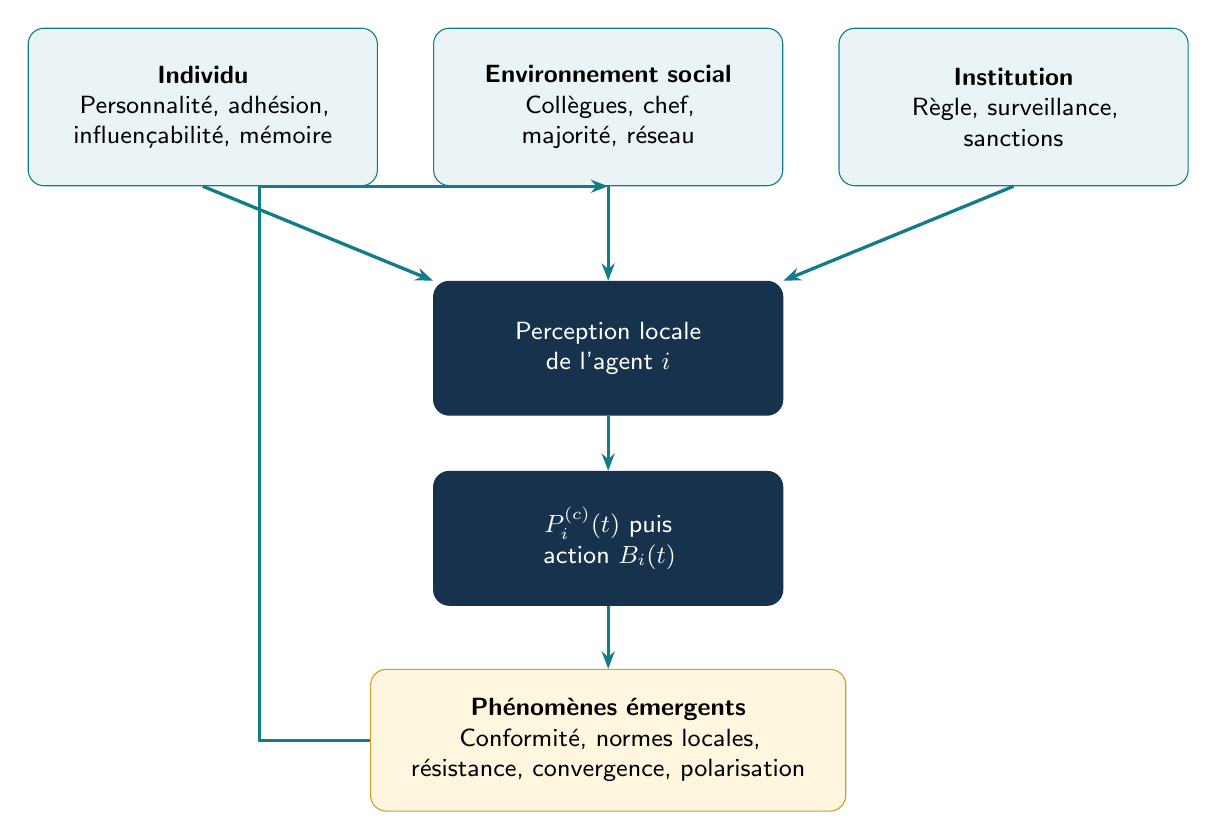
\begin{tikzpicture}[
  every node/.style={font=\sffamily\small,align=center},
  box/.style={rectangle,rounded corners=2mm,draw=Teal,fill=Ice,
    text width=42mm,minimum height=20mm},
  core/.style={rectangle,rounded corners=2mm,draw=Navy,fill=Navy,
    text=white,text width=42mm,minimum height=17mm},
  resultbox/.style={rectangle,rounded corners=2mm,draw=Gold,fill=SoftGold,
    text width=58mm,minimum height=18mm},
  arrow/.style={-{Stealth[length=2.2mm]},very thick,color=Teal}
]
\node[box] (ind) {\textbf{Individu}\\Personnalité, adhésion,\\influençabilité, mémoire};
\node[box,right=7mm of ind] (soc) {\textbf{Environnement social}\\Collègues, chef,\\majorité, réseau};
\node[box,right=7mm of soc] (ins) {\textbf{Institution}\\Règle, surveillance,\\sanctions};
\node[core,below=12mm of soc] (per) {Perception locale\\de l’agent $i$};
\node[core,below=7mm of per] (pro) {$P_i^{(c)}(t)$ puis\\action $B_i(t)$};
\node[resultbox,below=8mm of pro] (out) {\textbf{Phénomènes émergents}\\Conformité, normes locales,\\résistance, convergence, polarisation};
\draw[arrow] (ind.south) -- (per.north west);
\draw[arrow] (soc.south) -- (per.north);
\draw[arrow] (ins.south) -- (per.north east);
\draw[arrow] (per)--(pro);
\draw[arrow] (pro)--(out);
\draw[arrow] (out.west) -- ++(-14mm,0) |- (soc.south);
\end{tikzpicture}
\caption{Architecture logique du modèle}
\label{fig:architecture}
\end{figure}

\begin{keybox}[title=Principe fondamental]
\[
\begin{gathered}
\text{mécanismes individuels}+\text{interactions locales}+\text{institution}\\
\Downarrow\\[-1mm]
\text{décisions probabilistes}\longrightarrow\text{résultats collectifs}.
\end{gathered}
\]
Le résultat macroscopique doit être observé, analysé et validé ; il ne doit
jamais être imposé dans le code.
\end{keybox}

\clearpage
\appendix
\section{Pseudocode de référence}

\begin{tcolorbox}[
  enhanced,breakable,
  colback=Ink,colframe=Ink,
  coltext=white,
  fontupper=\ttfamily\small,
  arc=1mm,left=4mm,right=4mm,top=3mm,bottom=3mm]
pour chaque graine r :\par
\quad initialiser agents, services, traits et réseau\par
\quad sauvegarder l'état initial commun\par
\quad pour phase dans \{1, 2, 3\} :\par
\qquad restaurer l'état initial commun\par
\qquad configurer règle, surveillance et sanction\par
\qquad tirer B(0) avec la même graine appariée\par
\qquad pour t = 1 ... T :\par
\qquad\quad pour chaque agent i :\par
\qquad\qquad observer B(t-1), voisins, chef si employé et sanctions visibles\par
\qquad\qquad calculer SI\_i(t), M\_i(t) et risque\_perçu\_i(t)\par
\qquad\qquad calculer Z\_i(t) puis P\_i(conforme,t)\par
\qquad\qquad tirer le comportement candidat B\_i(t)\par
\qquad\quad appliquer simultanément tous les B\_i(t)\par
\qquad\quad si surveillance active :\par
\qquad\qquad détecter les violations avec probabilité p\_d\par
\qquad\qquad appliquer la sanction graduée et mettre à jour V\_i\par
\qquad\quad enregistrer sorties individuelles, services et organisation\par
\quad comparer les phases par différences appariées\par
\end{tcolorbox}

\section{Dictionnaire minimal des paramètres}

\begin{longtable}{L{29mm}L{45mm}L{64mm}}
\toprule
\rowcolor{Navy}
\color{white}\textbf{Nom de code} &
\color{white}\textbf{Symbole} &
\color{white}\textbf{Description}\\
\midrule
\endfirsthead
\toprule
\rowcolor{Navy}
\color{white}\textbf{Nom de code} &
\color{white}\textbf{Symbole} &
\color{white}\textbf{Description}\\
\midrule
\endhead
\code{population\_size} & $N$ & Nombre total d’agents.\\
\code{manager\_share} & $N_H/N$ & Part de chefs.\\
\code{periods} & $T$ & Durée de l’exécution.\\
\code{employee\_degree} & $k_i^E$ & Nombre cible de relations entre employés.\\
\code{manager\_degree} & $k_i^H$ & Nombre cible de relations entre chefs.\\
\code{within\_group\_prob} & $p_{\mathrm{intra}}$ & Part attendue de liens internes.\\
\code{peer\_weight} & $w_c$ & Poids d’un collègue.\\
\code{manager\_weight} & $w_h$ & Poids du chef.\\
\code{memory\_decay} & $\lambda$ & Persistance de la mémoire.\\
\code{detection\_}\newline\code{probability} & $p_d$ & Risque réel de détection.\\
\code{sanction\_levels} & $(\ell_1,\ell_2,\ell_3)$ &
Niveaux : $(0{,}25;0{,}50;1{,}00)$.\\
\code{risk\_update\_}\newline\code{weights} & $(\alpha,\gamma)$ &
Poids personnel et observé : $(0{,}40;0{,}40)$.\\
\code{rule\_weight} & $\beta_R$ & Contribution de la règle.\\
\code{social\_weight} & $\beta_I$ & Contribution de l’influence sociale.\\
\code{sanction\_weight} & $\beta_S$ & Contribution du risque de sanction.\\
\code{random\_seed} & $r$ & Graine de reproductibilité.\\
\bottomrule
\end{longtable}

\clearpage
\begin{thebibliography}{99}
\addcontentsline{toc}{section}{Références}

\bibitem{grimm2020}
V. Grimm \emph{et al.}, ``The ODD protocol for describing agent-based and other
simulation models: A second update to improve clarity, replication, and
structural realism,'' \emph{Journal of Artificial Societies and Social
Simulation}, vol. 23, no. 2, art. no. 7, 2020,
doi: \href{https://doi.org/10.18564/jasss.4259}{10.18564/jasss.4259}.

\bibitem{epstein1996}
J. M. Epstein and R. L. Axtell, \emph{Growing Artificial Societies: Social
Science from the Bottom Up}. Washington, DC, USA: Brookings Institution Press;
Cambridge, MA, USA: MIT Press, 1996.

\bibitem{gilbert2005}
N. Gilbert and K. G. Troitzsch, \emph{Simulation for the Social Scientist},
2nd ed. Maidenhead, U.K.: Open University Press, 2005.

\bibitem{costa1992}
P. T. Costa, Jr. and R. R. McCrae, \emph{Revised NEO Personality Inventory
(NEO PI-R) and NEO Five-Factor Inventory (NEO-FFI): Professional Manual}.
Odessa, FL, USA: Psychological Assessment Resources, 1992.

\bibitem{bandura1977}
A. Bandura, \emph{Social Learning Theory}. Englewood Cliffs, NJ, USA:
Prentice-Hall, 1977.

\bibitem{cialdini2009}
R. B. Cialdini, \emph{Influence: Science and Practice}, 5th ed. Boston, MA,
USA: Pearson, 2009.

\bibitem{simon1997}
H. A. Simon, \emph{Administrative Behavior: A Study of Decision-Making
Processes in Administrative Organizations}, 4th ed. New York, NY, USA:
Free Press, 1997.

\bibitem{ostrom1990}
E. Ostrom, \emph{Governing the Commons: The Evolution of Institutions for
Collective Action}. Cambridge, U.K.: Cambridge University Press, 1990,
doi: \href{https://doi.org/10.1017/CBO9780511807763}
{10.1017/CBO9780511807763}.

\bibitem{axelrod2006}
R. Axelrod, \emph{The Evolution of Cooperation}, rev. ed. New York, NY, USA:
Basic Books, 2006.

\bibitem{schelling2006}
T. C. Schelling, \emph{Micromotives and Macrobehavior}, rev. ed. New York,
NY, USA: W. W. Norton \& Company, 2006.

\bibitem{schruben2011}
L. W. Schruben, ``Common random numbers,'' in \emph{Wiley Encyclopedia of
Operations Research and Management Science}, J. J. Cochran, Ed. Hoboken, NJ,
USA: Wiley, 2011, doi:
\href{https://doi.org/10.1002/9780470400531.eorms0166}
{10.1002/9780470400531.eorms0166}.

\end{thebibliography}

\end{document}
